%\documentclass[mathserif]{beamer}
\documentclass[handout]{beamer}
%\usetheme{Goettingen}
%\usetheme{Warsaw}
\usetheme{Singapore}



%\usetheme{Frankfurt}
%\usetheme{Copenhagen}
%\usetheme{Szeged}
%\usetheme{Montpellier}
%\usetheme{CambridgeUS}
%\usecolortheme{}
%\setbeamercovered{transparent}
\usepackage[english, activeacute]{babel}
\usepackage[utf8]{inputenc}
\usepackage{amsmath, amssymb}
\usepackage{dsfont}
\usepackage{graphics}
\usepackage{cases}
\usepackage{graphicx}
\usepackage{pgf}
\usepackage{epsfig}
\usepackage{amssymb}
\usepackage{multirow}	
\usepackage{amstext}
\usepackage{algorithm2e}
\usepackage{amsmath}
\usepackage{epic}
\usepackage{epsfig}
\usepackage{fontenc}
\usepackage{framed,color}
\usepackage{palatino, url, multicol}
%\algsetup{indent=2em}
\newcommand{\factorial}{\ensuremath{\mbox{\sc Factorial}}}
\newcommand{\BIGOP}[1]{\mathop{\mathchoice%
{\raise-0.22em\hbox{\huge $#1$}}%
{\raise-0.05em\hbox{\Large $#1$}}{\hbox{\large $#1$}}{#1}}}
\newcommand{\bigtimes}{\BIGOP{\times}}
\vspace{-0.5cm}
\title{Acquiring and Exploiting Lexical Knowledge for Twitter Sentiment Analysis}
\vspace{-0.5cm}
\author[Felipe Bravo Márquez]{\footnotesize
%\author{\footnotesize  
 \textcolor[rgb]{0.00,0.00,1.00}{Felipe Bravo-Marquez} \\ Chief Supervisor: Bernhard Pfahringer \\  Supervisor: Eibe Frank} 
  
 
%\vspace{-0.3cm}
\institute{Department of Computer Science, University of Waikato }

\titlegraphic{\includegraphics[scale=0.3]{../../img/waikato.png}}



\date{21 September,2016}

\begin{document}
\begin{frame}
\titlepage


\end{frame}

\section{Introduction}

\begin{frame}{Social Media}
\begin{scriptsize}
\begin{itemize}
 \item Microblogging services are increasingly being adopted by people in order to access and publish information.  
 \item \textbf{Twitter}: Massively used Microblogging platform where users post messages (a.k.a \textbf{tweets}) limited to 140 characters. 
 \item Tweets use a unique \textbf{informal dialect} including many abbreviations, acronyms, misspelled words, hashtags, and emoticons, e.g., \textbf{lol}, \textbf{omg}, \textbf{hahaha}, \textbf{\#hatemonday}, \textbf{\#SweetAsBro}, \textbf{\#yeahnah}, \textbf{:)} .
\end{itemize}
  \begin{figure}[h]
        	
\includegraphics[scale = 0.2]{pics/twitter.png}
        \end{figure}

\end{scriptsize}
\end{frame}



\begin{frame}{Sentiment Analysis and Social Media}
\begin{scriptsize}
\begin{itemize}
 \item  Twitter users tend to publish \textbf{personal opinions} regarding certain topics and news events. 
 
 \begin{enumerate}
  \footnotesize{
  \item Hey @Apple, pretty much all your products are amazing.  You blow minds every time you launch a new gizmo. That said, your hold music is crap.
 \item \#windows sucks...  I want \#imac so bad!!!  why is it so damn expensive :( @apple please give me free imac and I will love you :D}
 \end{enumerate}

 
 \item Analysing the sentiment underlying these opinions has important applications in product \textbf{marketing} and \textbf{politics}.
 
   \begin{figure}[h]
        	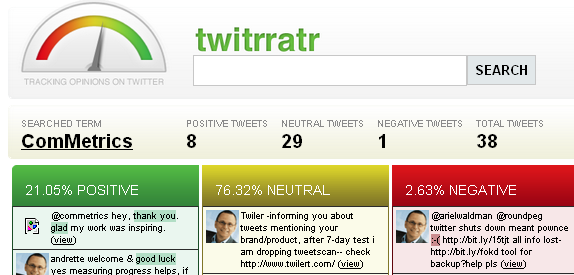
\includegraphics[scale = 0.4]{pics/tweetOpinions.png}
        \end{figure}
\end{itemize}
\end{scriptsize}

\end{frame}


\begin{frame}{Opinion Mining or Sentiment Analysis}
\begin{scriptsize}\begin{itemize}
 \item Application of \textbf{NLP} and \textbf{text mining} techniques to identify and extract subjective information from textual datasets.
\end{itemize}

\begin{block}{Main Problem: Message-level Polarity Classification (MPC)}
  \begin{enumerate}
   \item Automatically classify a tweet to classes \textcolor[rgb]{0.00,0.00,1.00}{\textbf{positive}}, \textcolor[rgb]{1.00,0.00,0.00}{\textbf{negative}}, or \textcolor[rgb]{0.00,1.00,0.00}{\textbf{neutral}}. 
   
     \begin{figure}[h]
        	
\includegraphics[scale = 0.15]{pics/sent.png}
        \end{figure}
   
   \item State-of-the-art solutions use \textbf{supervised} machine learning models trained from \textbf{manually} annotated examples \cite{NRCJAIR14}.
  \end{enumerate} 
\end{block}

\end{scriptsize}

\end{frame}

\begin{frame}{Drawbacks of Supervised models for MPC}
\begin{scriptsize}
  \begin{itemize}
   \item \textbf{Label sparsity (LS)}: manual annotation is \textbf{labour-intensive} and \textbf{time-consuming}. 
   \item \textbf{Concept drift}: the sentiment pattern can vary from one collection to another (domain-drift, temporal-drift).
  \end{itemize} 

A classifier trained from tweets annotated for one domain will \textbf{not necessarily} work on another one!

\begin{block}{Examples of domain-Drift}
\begin{enumerate}
\item  For me the queue was pretty \textcolor[rgb]{0.00,0.00,1.00}{\textbf{small}} and it was only a 20 minute wait I think but was so worth it!!! :D @raynwise
\item Odd spatiality in Stuttgart. Hotel room is so  \textcolor[rgb]{1.00,0.00,0.00}{\textbf{small}} I can barely turn around but surroundings are inhumanly vast \& long under construction.
\end{enumerate}
\end{block}


\end{scriptsize}

\end{frame}




\begin{frame}{Solutions to MPC with LS}
\begin{scriptsize}
\begin{block}{Using Prior Lexical Knowledge}
  \begin{itemize}
  \item An opinion lexicon is a lists of terms labelled by sentiment.
\item They are normally composed of positive and negative words such as \textcolor[rgb]{0.00,0.00,1.00}{\textbf{happy, wonderful}} and \textcolor[rgb]{1.00,0.00,0.00}{\textbf{sad, bad}}.
\item Can be used for \textbf{unsupervised} sentiment classification \cite{ThelwallBP12}, or as \textbf{low-dimensional} features~\cite{kouloumpis2011twitter}.   
\item Informal Twitter words are \textbf{not} covered by most popular lexicons.
\item The manual creation of a Twitter-oriented opinion lexicon is a \textbf{time-consuming} task.
  \end{itemize} 
\end{block}

\end{scriptsize}

\end{frame}

\begin{frame}{Solutions to MPC with LS (2)}
\begin{scriptsize}
\begin{block}{Distant Supervision}
  \begin{itemize}
   \item Automatically \textbf{label} unlabelled data (\textbf{Twitter API}) using a heuristic method~\cite{Mintz2009}.
   \item \textbf{Emoticon-Annotation Approach (EAA)}: tweets with positive \textcolor[rgb]{0.00,0.00,1.00}{\textbf{:)}} or negative \textcolor[rgb]{1.00,0.00,0.00}{\textbf{:(}} emoticons are labelled according to the polarity indicated by the emoticon~\cite{Read2005}.
  \item The emoticon is \textbf{removed} from the content.
\item Drawback: emoticons are \textbf{rarely} used in certain domains such as politics. 
    \end{itemize} 


    
\end{block}
\end{scriptsize}

\end{frame}





\begin{frame}{Research Problem}

This thesis addresses the label sparsity problem for Twitter sentiment classification by automatically building \textbf{two type of resources}. 
\begin{enumerate}
 \item \textbf{Twitter-specific opinion lexicons}: we develop machine learning models to induce polarity lexicons from tweets. 
 \item  \textbf{Synthetically labelled tweets}: we develop distant supervision methods based on \textbf{lexical knowledge} (we go beyond emoticons). 
 \end{enumerate}

\end{frame}


\section{Polarity Lexicon Induction}


\begin{frame}{Previous work on Polarity Lexicon Induction (PLI)}
\begin{scriptsize}

\begin{itemize} 
 \item The acquisition is normally done by exploiting \textbf{relations} between a \textbf{small seed lexicon} and \textbf{unknown words} from a \textbf{knowledge} resource.
\item  Two type of resources can be used: a \textbf{semantic network} (structured) such as \textbf{WordNet}, or a \textbf{corpus of documents} (unstructured). 
\end{itemize}



\begin{figure}[h!]
	\centering
	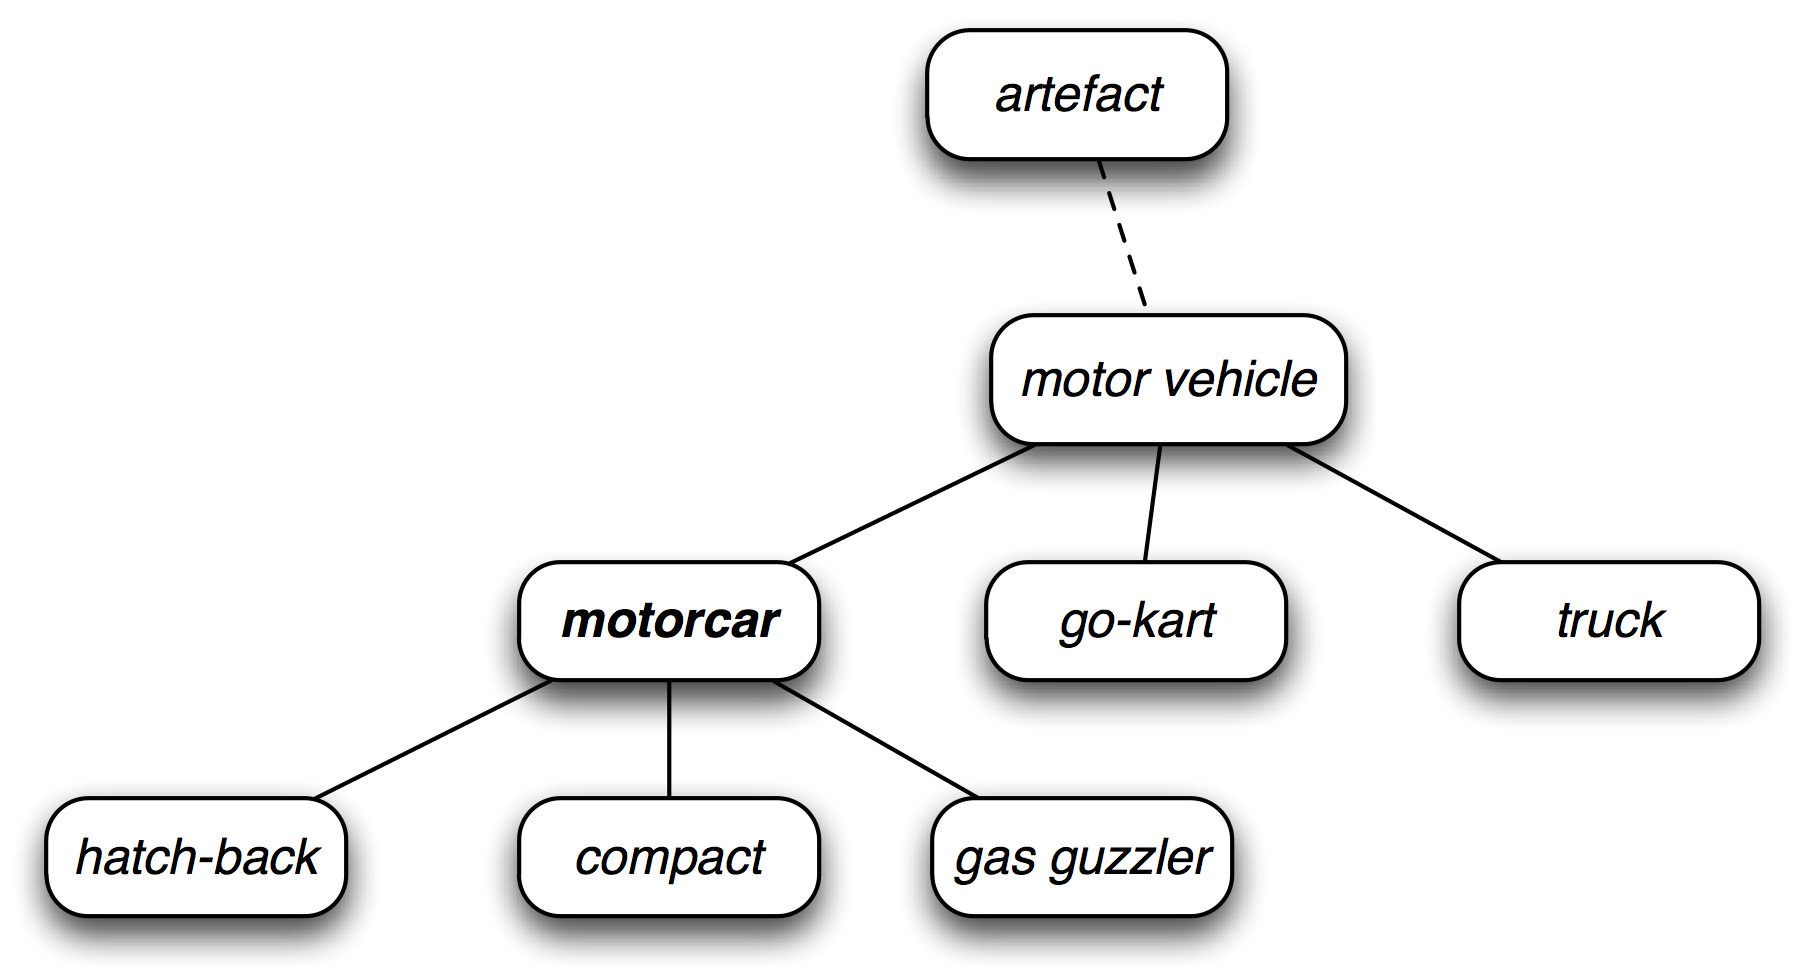
\includegraphics[scale=0.3]{pics/wordnet.png}
\end{figure}

\begin{figure}[h!]
	\centering
	
\includegraphics[scale=0.2]{pics/documents.jpg}
\end{figure}





\end{scriptsize}
\end{frame}



\begin{frame}{PLI using Semantic Networks}
\begin{scriptsize}

\begin{itemize} 
\item Methods based on WordNet expand the seed words using semantic relations such \textbf{synonyms} and \textbf{antonyms}, \cite{Liu2004,Kim2004}.
\item Hypothesis: synonyms have the \textbf{same} polarity and antonyms have the \textbf{opposite}.
\item In \cite{kamps2004} a \textbf{graph} was created using WordNet \textbf{adjectives} as vertices and the \textbf{synonym} relation as edges. 
\item Words are expanded by its \textbf{relative distance} from the two seed terms \textbf{good} and \textbf{bad}.
\item In \cite{Esuli2005, esuli2006} the authors take the \textbf{dictionary definitions} of the seed words to train a word-level classifier. 
\item As semantic networks cover a fixed vocabulary, they \textbf{cannot} capture informal Twitter words. 
\end{itemize}
\end{scriptsize}
\end{frame}



\begin{frame}{Corpus-based PLI}
\begin{scriptsize}
\begin{itemize}
\item Corpus approaches exploit \textbf{statistical patterns} observed in document corpora (e.g.\textbf{tweets}). 
\item Turney et.al proposed an unsupervised measure called \textbf{PMI semantic orientation} (PMI-SO) \cite{turney2003measuring}.
\item It is calculated as the difference between the point-wise mutual information \textbf{PMI} of the word with a positive and a negative variable $y$.

\begin{displaymath}
  \operatorname{PMI-SO}(w) = log_2 \left( \frac{\operatorname{count}(w \wedge y=pos) \times \operatorname{count}(y=neg)}{\operatorname{count}(y=pos)\times\operatorname{count}(w\wedge y=neg)}\right)
\end{displaymath}
\item For Twitter PLI these variables correspond to message-level labels obtained using \textbf{EAA} \cite{Mohammad2013, Zhou2014}
\item The approach suffers from the same limitations as \textbf{EAA} for MPC. 
\end{itemize}
\end{scriptsize}
\end{frame}



\begin{frame}{Word-sentiment Associations for PLI}
\begin{scriptsize}
\begin{itemize}
\item We propose a \textbf{supervised framework} for \textbf{PLI} based on \textbf{sentiment-annotated tweets}.
\item The tweets are labelled in an \textbf{automatic fashion} (EAA and transfer model). 
\item Each expanded word has a \textbf{probability distribution}, describing how positive, negative, and neutral it is.
\item All the entries of the lexicon are associated with a corresponding \textbf{part-of-speech} tag.
\item This is useful for word \textbf{disambiguation} e.g., fine can be an adjective or a noun.
\item These properties are inspired by \textbf{SentiWordnet}.
\end{itemize}
\end{scriptsize}

\end{frame}

\begin{frame}{Methodology}
\begin{figure}[htb]
	\centering
	 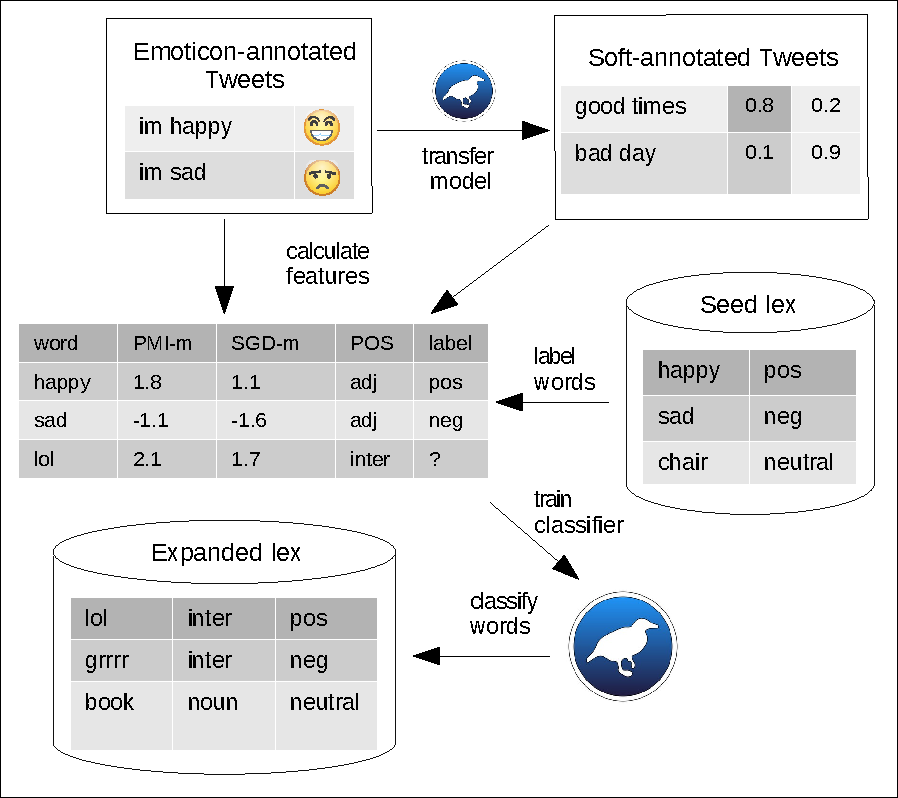
\includegraphics[scale=0.5]{pics/diagramcrop.pdf}
	\label{fig:sosgd}
\end{figure}
\end{frame}



\begin{frame}{Ground-Truth word polarities}
\begin{scriptsize}
\begin{itemize}
\item The expansion requires a \textbf{seed lexicon} with words labelled by sentiment.
\item We create a meta-lexicon by taking the \textbf{union} of existing hand-made lexicons.
\item We discard all words where a \textbf{polarity clash} is observed.
\end{itemize}


\begin{table}[htbp]
\begin{center}
\begin{tabular}{l|c|c|c}
\hline
 & Positive & Negative & Neutral \\ \hline
AFINN & 564 & 964 & 0 \\ 
Bing Liu & 2003 & 4782 & 0 \\ 
MPQA & 2295 & 4148 & 424 \\ 
NRC-Emo & 2312 & 3324 & 7714 \\ \hline
Seed Lexicon & 3730 & 6368 & 7088 \\ \hline
\end{tabular}
\end{center}
\caption{Lexicon Statistics}
\label{tab:lexstats}
\end{table}
\end{scriptsize}
\end{frame}



\begin{frame}{Word-level Features}
\begin{scriptsize}
\begin{itemize}
\item We prepend a \textbf{POS-tag} prefix to each word in order to differentiate \textbf{homographs} exhibiting different POS-tags and use the POS tag as a nominal feature.

\item We calculate two types of associations  for each word: \textbf{Stochastic Gradient Descent} (SGD-SO), and \textbf{PMI Semantic Orientation} (PMI-SO).

\item We calculate associations from \textbf{hard} and \textbf{soft} message-level labels.

\end{itemize}
\end{scriptsize}

\end{frame}




\begin{frame}{The SGD-SO association }
\begin{scriptsize}
\begin{itemize}
\item  This SGD-SO association is calculated by incrementally training a \textbf{linear support vector machine} from the collection of \textbf{hard-labelled} tweets.
\item We use \textbf{stochastic gradient descent} (SGD) online learning process.
\begin{equation}\label{eq:sgd}
\frac{\lambda}{2}||w||^2+\sum [1- y (\mathbf{xw} +b) ]_{+}.
\end{equation}
\item We use a squared loss function over the log odds $z=\operatorname{log}_2(\frac{pos(d)}{neg(d)})$ for \textbf{soft-annotated} tweets.
\begin{equation}\label{eq:sgdSQ}
\frac{\lambda}{2}||w||^2+\sum (z - (\mathbf{xw} +b))^2.
\end{equation}

\end{itemize}
\end{scriptsize}

\end{frame}


\begin{frame}{The PMI-SO association}
\begin{scriptsize}
\begin{itemize}
\item  The second association for \textbf{hard-annotated} tweets corresponds to the \textbf{PMI semantic orientation} (PMI-SO).

\begin{equation}\label{eq:so}
 \operatorname{PMI-SO}(w) = log_2 \left( \frac{\operatorname{count}(w \wedge y=1) \times \operatorname{count}(y=-1)}{ \operatorname{count}(y=1) \times \operatorname{count}(w\wedge y=-1)}\right)
\end{equation}

\item For soft-annotated tweets:
\begin{equation}\label{eq:so_soft}
 \operatorname{PMI-SO}'(w) = log_2 \left( \frac{ \sum_{d \in C(w)} \operatorname{pos}(d) \times \sum_{d \in C} \operatorname{neg}(d)}{ \sum_{d \in C} \operatorname{pos}(d) \times \sum_{d \in C(w)} \operatorname{neg}(d)}\right)
\end{equation}


\end{itemize}
\end{scriptsize}

\end{frame}


\begin{frame}{Feature Visualisation}
\begin{scriptsize}
\begin{figure}[htb]
	\centering
	 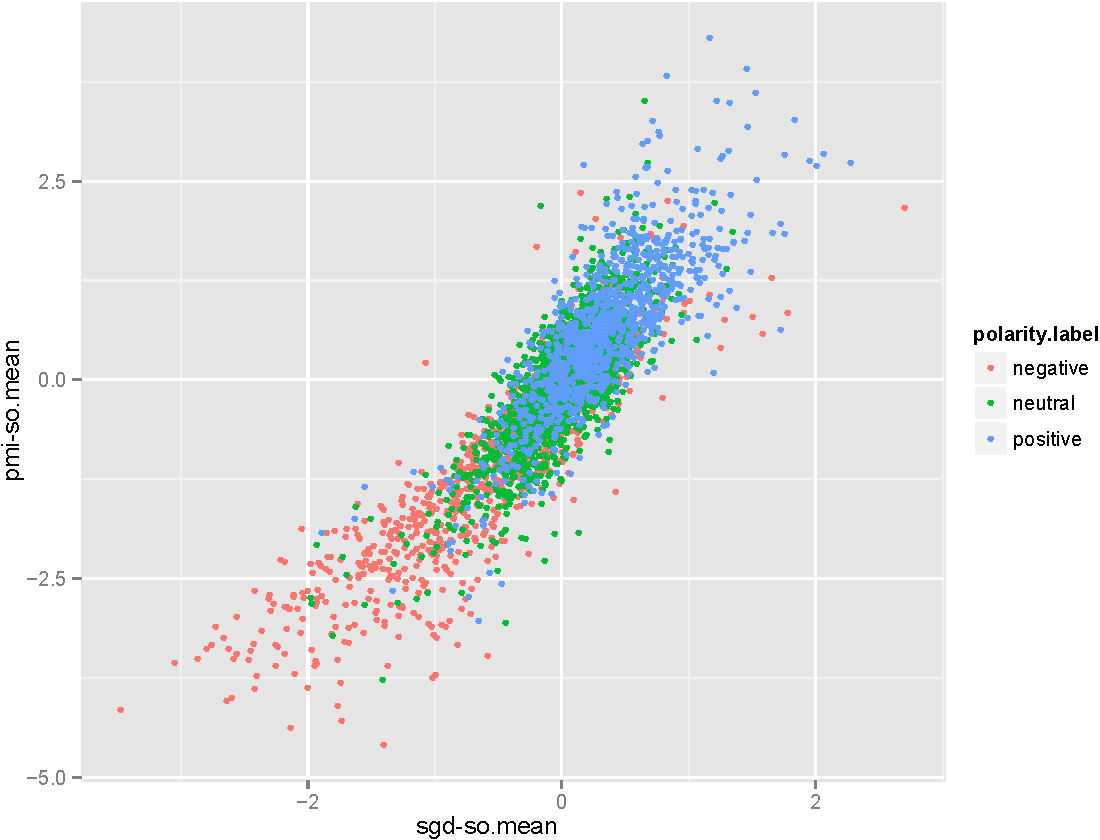
\includegraphics[width=7.5cm,height=6cm]{pics/SGDSO-new.pdf}
	\caption{PMI-SO vs SGD-SO scatterplot.}
	\label{fig:sosgd}
\end{figure}
\end{scriptsize}

\end{frame}


\begin{frame}{Word-level Classification Results using RBF SVMs}
\footnotesize
\begin{table}[!htb]
\begin{center}
\begin{tabular}{l|l|l}
\hline \hline
\multicolumn{ 3}{c}{Weighted AUC } \\ \hline \hline
Dataset & PMI-SO & ALL FEATURES \\ \hline
ED.EM & 0.62 $\pm$ 0.02 &  \textbf{0.65 $\pm$ 0.02} $+$ \\  
STS & 0.64 $\pm$ 0.02 & \textbf{0.66 $\pm$ 0.01} $+$   \\ 
%ED.T07 & 0.62 $\pm$ 0.02 & \textbf{0.65 $\pm$ 0.02} $+$   \\ 
ED.SL &  0.63 $\pm$ 0.02 & \textbf{0.65  $\pm$  0.02} $+$ \\ \hline 
\end{tabular}
\end{center}
\caption{World-level classification performance.} 
\label{tab:classres}
\end{table}
\end{frame}

\begin{frame}{Expanded Lexicon}
\begin{figure}[ht]
\begin{center}
\begin{tabular}{cc}
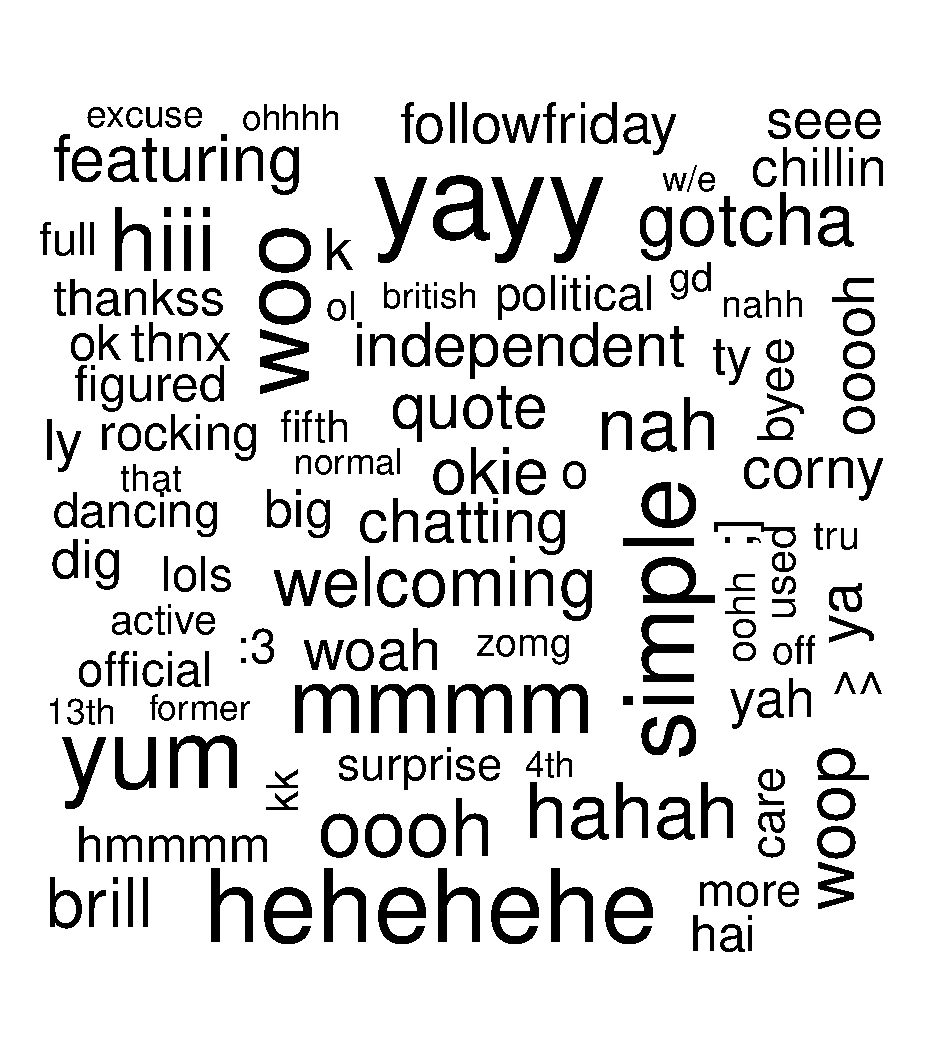
\includegraphics[scale=0.25]{../poswords.pdf}
&
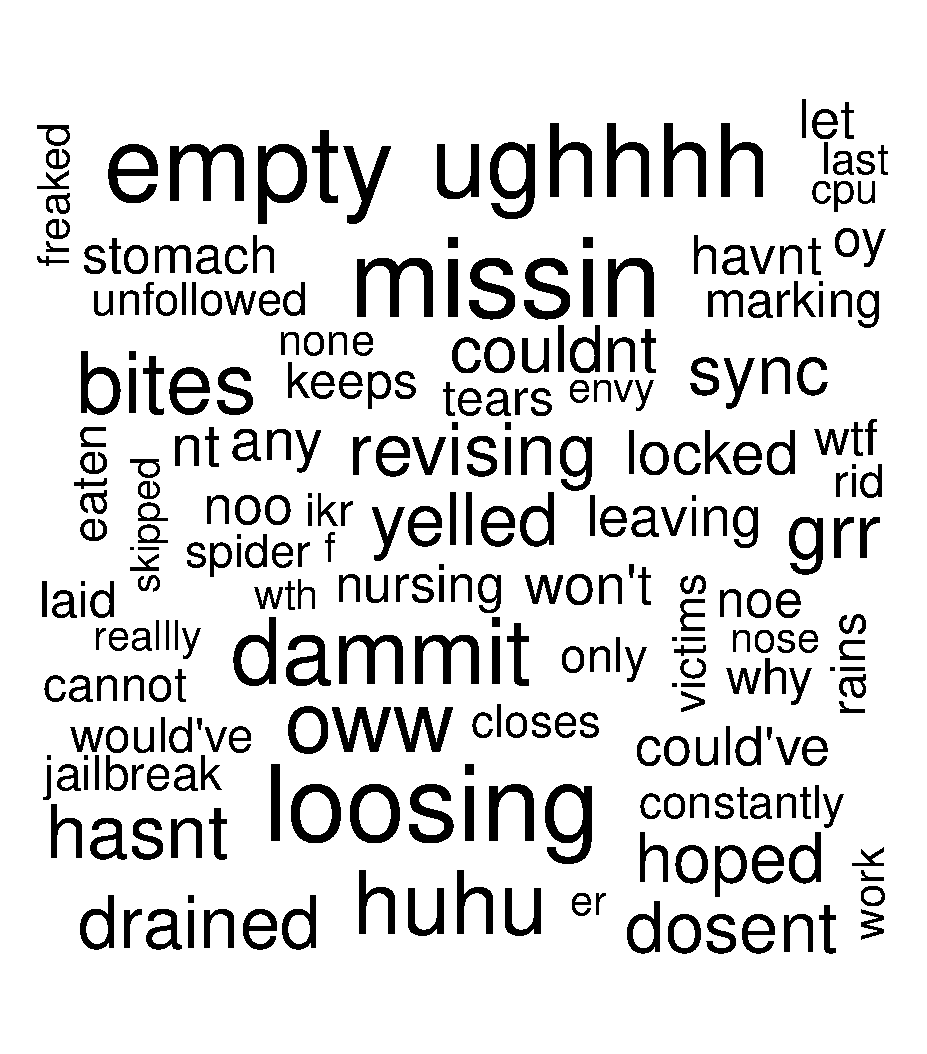
\includegraphics[scale=0.25]{../negwords.pdf}\\
(a) & (b)  
\end{tabular}
\caption{Word clouds of positive and negative words using log odds proportions.}
\label{fig:wordcloud}
\end{center}
\end{figure}
\end{frame}


\begin{frame}{Message-level classification}


\begin{table}[htbp]
\begin{center}
\scalebox{0.8}{
\begin{tabular}{l|l@{\hspace{0.1cm}}l@{\hspace{0.1cm}}l@{\hspace{0.1cm}}l@{\hspace{0.1cm}}l@{\hspace{0.1cm}}l@{\hspace{0.1cm}}|l@{\hspace{0.1cm}}l@{\hspace{0.1cm}}l@{\hspace{0.1cm}}l@{\hspace{0.1cm}}l@{\hspace{0.1cm}}l@{\hspace{0.1cm}}|l@{\hspace{0.1cm}}l@{\hspace{0.1cm}}l@{\hspace{0.1cm}}l@{\hspace{0.1cm}}l@{\hspace{0.1cm}}l@{\hspace{0.1cm}}}
\hline \hline
\multicolumn{1}{c}{} &\multicolumn{18}{c}{ AUC}\\ \hline \hline
Dataset & \multicolumn{6}{c|}{6HumanCoded} & \multicolumn{6}{c|}{Sanders} & \multicolumn{6}{c}{SemEval} \\ \hline
Seed.Lex & 0.77 & $\pm$ & 0.03 & = & + & - & 0.77 & $\pm$ & 0.04 & = & + & = & 0.77 & $\pm$ & 0.02 & = & + & -\\ 
SW & 0.74 & $\pm$ & 0.03 & - & = & - & 0.7 & $\pm$ & 0.05 & - & = & - & 0.76 & $\pm$ & 0.02 & = & = & - \\ 
SS & 0.81 & $\pm$ & 0.02 & + & + & = & 0.78 & $\pm$ & 0.03 & = & + & = & 0.81 & $\pm$ & 0.02 & + & + & = \\ \hline
STS & 0.82 & $\pm$ & 0.02 &+& + & = & \textbf{0.84} & $\pm$ & 0.04 & + & + & + & \textbf{0.83} & $\pm$ & 0.02 & + & + & +\\ 
ED.EM & 0.82 & $\pm$ & 0.03 &+& + & = & 0.83 & $\pm$ & 0.04 &+& + & + & 0.81 & $\pm$ & 0.02 & + & + & = \\ 
ED.SL  & 0.81 & $\pm$ & 0.02 & + & + & = & 0.83 & $\pm$ & 0.04 & + & + & + & 0.81 & $\pm$ & 0.02 & + & + & =\\ 
%ED.T07 & 0.81 & $\pm$ & 0.03 & + & + & = & 0.83 &$\pm$& 0.04 & + & + & + & 0.82 & $\pm$ & 0.02 & + & + & +  \\ 
ENS & \textbf{0.83} & $\pm$ & 0.02 & + & + & = & \textbf{0.84} & $\pm$ & 0.04 & + & + & + & \textbf{0.83} & $\pm$ & 0.02 & + & + & + \\  \hline \hline
\end{tabular}}
\end{center}
\caption{Message-level polarity classification performance. Best result per column is given in bold.}
\label{tab:messclass}
\end{table}

\end{frame}





\begin{frame}{PLI from unlabelled Tweets}
\begin{scriptsize}
\begin{itemize}
\item We propose another supervised model for lexicon expansion referred to as the \textbf{tweet-centroid model (TCM)}.
\item The words are represented by \textbf{high-dimensional vectors} based on the context's where they occur. 
\item In contrast to the previous approach the expansion is done from \textbf{unlabelled tweets}.
\item It is inspired by the \textbf{Distributional Hypothesis} \cite{harris1954}: words occurring in the same \textbf{contexts} tend to have similar meanings.
\item Or equivalently: ``a word is characterized by the \textbf{company} it keeps".
\end{itemize}
\end{scriptsize}
\end{frame}


\begin{frame}{The Tweet Centroid Model (TCM) }
\begin{scriptsize}
\begin{itemize}
\item We treat a \textbf{whole tweet} as a word's context.
\item We model tweets as \textbf{vectors} using standard NLP features.
\item We use high-dimensional \textbf{unigrams}  $\overrightarrow{tb}$ and low-dimensional \textbf{word-clusters} $\overrightarrow{tc}$ to form the feature space.
\item The word cluster are trained from a corpus of tweets using the \textbf{Brown clustering} algorithm \cite{brown1992class}. 
\end{itemize}
\end{scriptsize}
\end{frame}


\begin{frame}{The Tweet Centroid Model (TCM) (2)}
\begin{scriptsize}
\begin{itemize}
\item The \textbf{word-tweet set} $\mathcal{M}(w)$ is the set of tweets from a corpus $\mathcal{C}_U$ in which the word $w$ is observed (posting list in IR):
\begin{equation}
\mathcal{M}(w)=\{ m: w \in m\}
\end{equation}
\item The TCM word vector $\overrightarrow{w}$ is the \textbf{centroid} of all tweet vectors in $\mathcal{M}(w)$.
\begin{equation}
w_j = \sum_{t \in \mathcal{M}(w)} \frac{x_j^{(t)}}{|\mathcal{M}(w)|}
\end{equation}

\end{itemize}
\end{scriptsize}
\end{frame}




\begin{frame}{Tweet-centroid Model}

\begin{figure}[htb]
	\centering
	 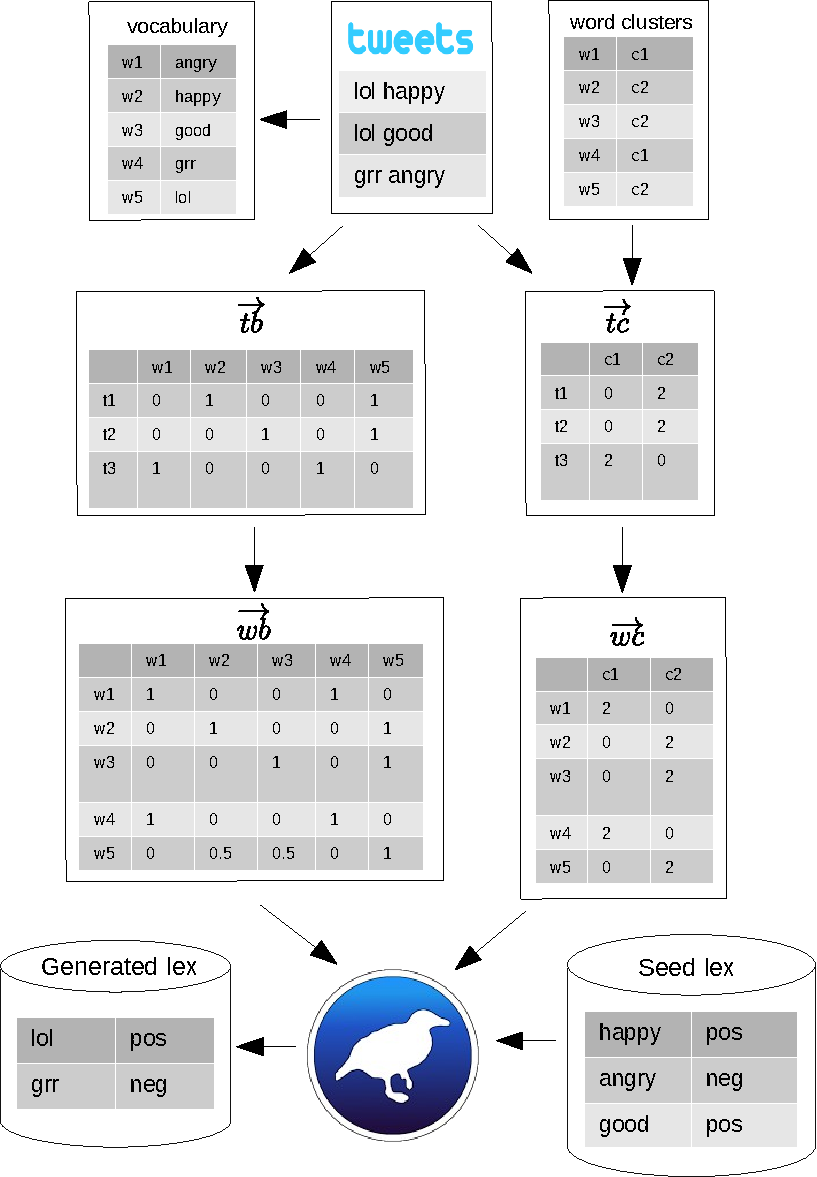
\includegraphics[scale=0.4]{sigirmodel.pdf}
\end{figure}



\end{frame}


\begin{frame}{Datasets}


\begin{table}[htbp]
\scriptsize
\begin{center}
\begin{tabular}{ l|r|r}
\hline \hline
Dataset & \multicolumn{1}{c|}{STS} & \multicolumn{1}{c}{ED} \\ \hline 
\#tweets & $1,600,000$ & $2,500,000$ \\ 
\#positive words & $2015$ & $2639$ \\ 
\#negative words & $2621$ & $3642$ \\ 
\#neutral words & $3935$ & $5085$ \\ 
\#unlabelled words & $36,451$ & $67,692$ \\ 
\#unigram attributes & $45,022$ & $79,058$ \\ 
\#word-clusters attributes & $993$ & $999$ \\ \hline \hline
\end{tabular}
\end{center}
\label{tab:corpstats}
\end{table}
\end{frame}

\begin{frame}{Word-level 3-class polarity classification performance}
\begin{scriptsize}
\begin{table}[!htb]
\scriptsize
\begin{center}
\begin{tabular}{l|c|c|c}
\hline \hline
\multicolumn{ 4}{c}{AUC} \\ \hline \hline
Dataset & Unigrams & Brown Clusters & Concatenation \\ \hline
%ED EM & 0.77 $\pm$ 0.01 & \textbf{0.79 $\pm$ 0.01} $+$ & \textbf{0.79 $\pm$ 0.01} $+$ \\
STS & 0.77 $\pm$ 0.01 & \textbf{0.79 $\pm$ 0.01} $+$ & \textbf{0.79 $\pm$ 0.01} $+$ \\ 
ED  & 0.78 $\pm$ 0.01 & 0.79 $\pm$ 0.01 $+$ & \textbf{0.80 $\pm$ 0.01} $+$ \\ 
\hline
\end{tabular}
\end{center}
\end{table}
\end{scriptsize}
\end{frame}


\begin{frame}{Message-level classification performance}
\begin{scriptsize}
 \begin{table}[htbp]
\scriptsize
\begin{center}
\begin{tabular}{l|c|c|c}
\hline \hline
\multicolumn{ 4}{c}{AUC} \\ \hline \hline
Dataset & Baseline & STS & ED \\ \hline
Sanders & 0.78 $\pm$ 0.04 & 0.80 $\pm$ 0.04 $+$ & \textbf{0.83 $\pm$ 0.04} $+$ \\ 
6-human & 0.79 $\pm$ 0.03 & 0.82 $\pm$ 0.03 $+$ & \textbf{0.83 $\pm$ 0.02} $+$ \\ 
SemEval & 0.78 $\pm$ 0.02 & 0.82 $\pm$ 0.02 $+$ & \textbf{0.84 $\pm$ 0.02} $+$ \\ \hline
\end{tabular}
\end{center}
\end{table}
\end{scriptsize}
\end{frame}



\begin{frame}{Other Applications of TCM}
\begin{scriptsize}
\begin{itemize}
\item  Multi-Label Classification of Emotions.
\end{itemize}

\begin{figure}[htbp]
\begin{center}
\scalebox{0.7}{
\begin{tabular}{cccc}
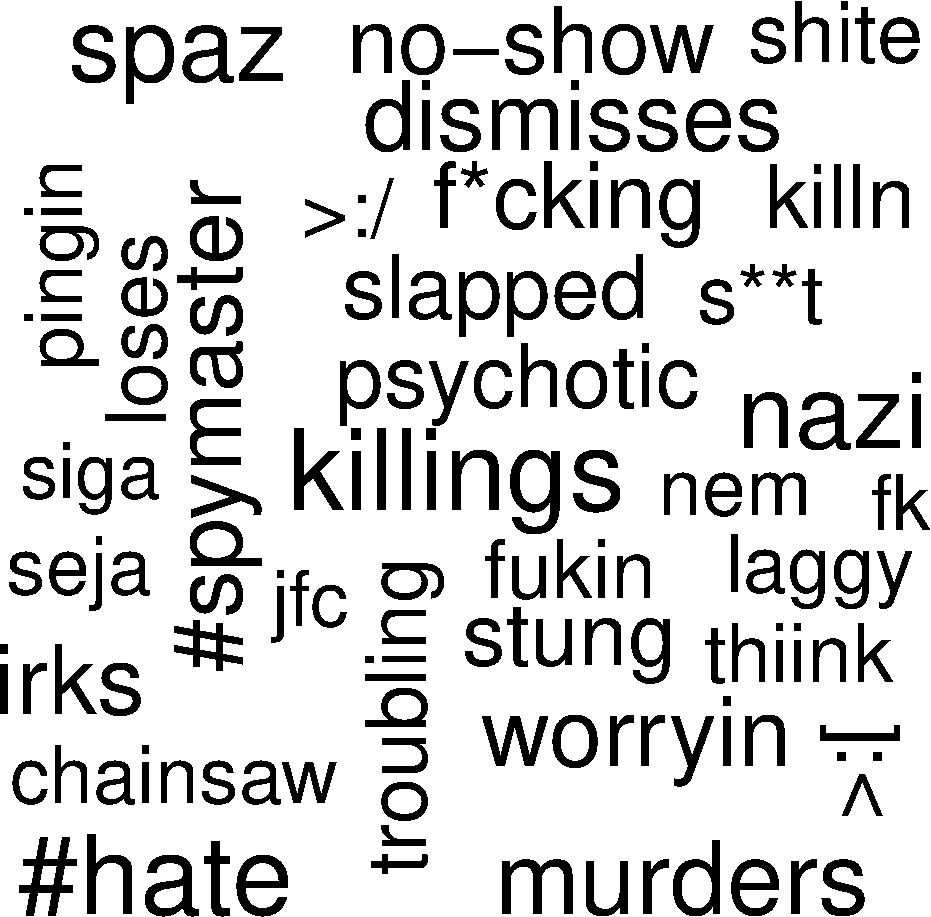
\includegraphics[scale=0.2]{pics/anger.pdf} & 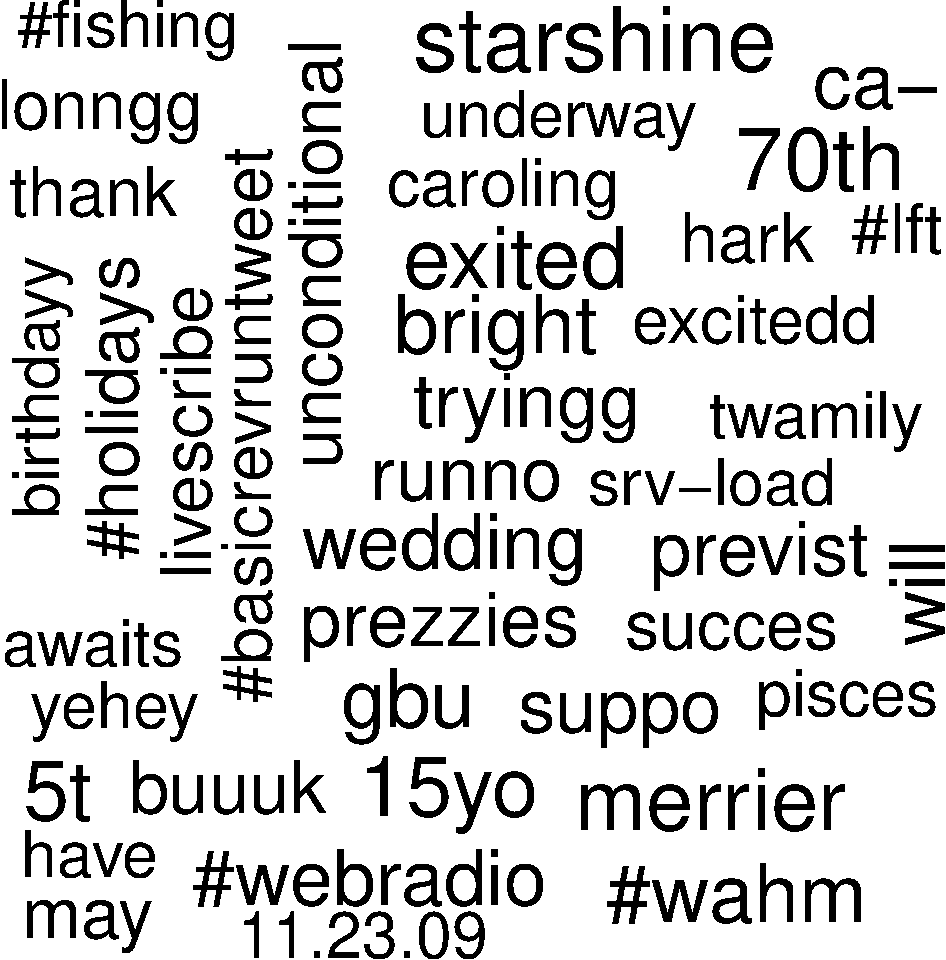
\includegraphics[scale=0.2]{pics/ant.pdf} & 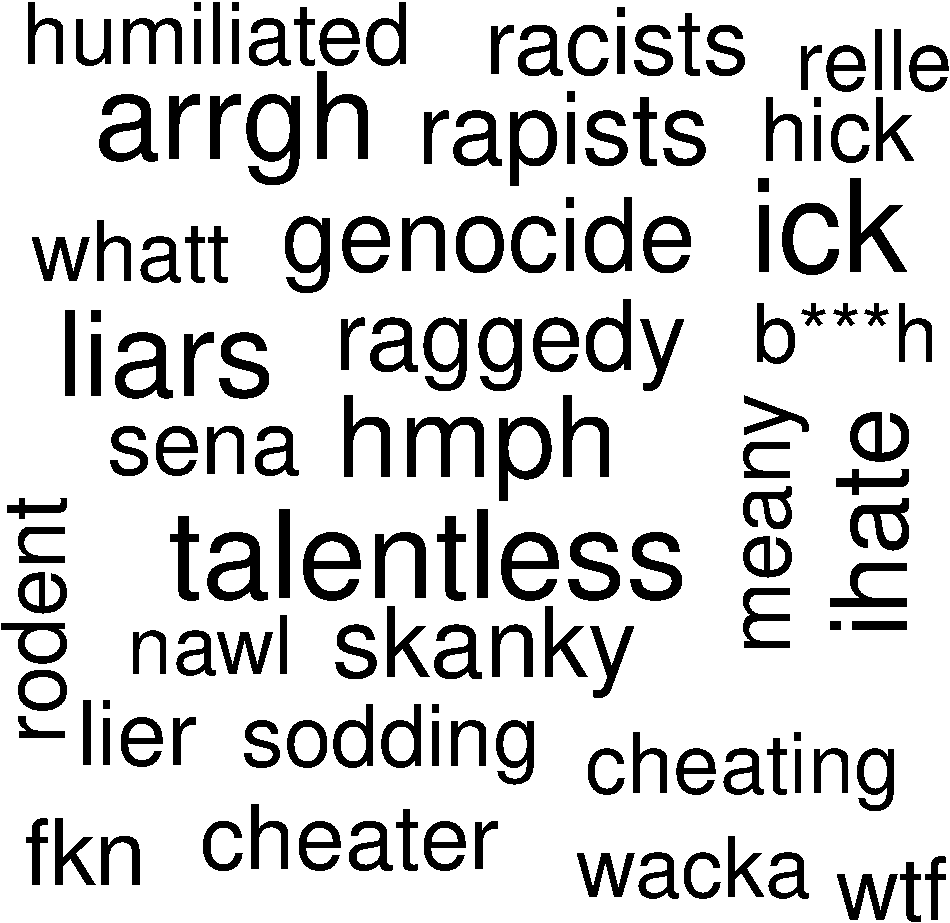
\includegraphics[scale=0.2]{pics/disg.pdf} & 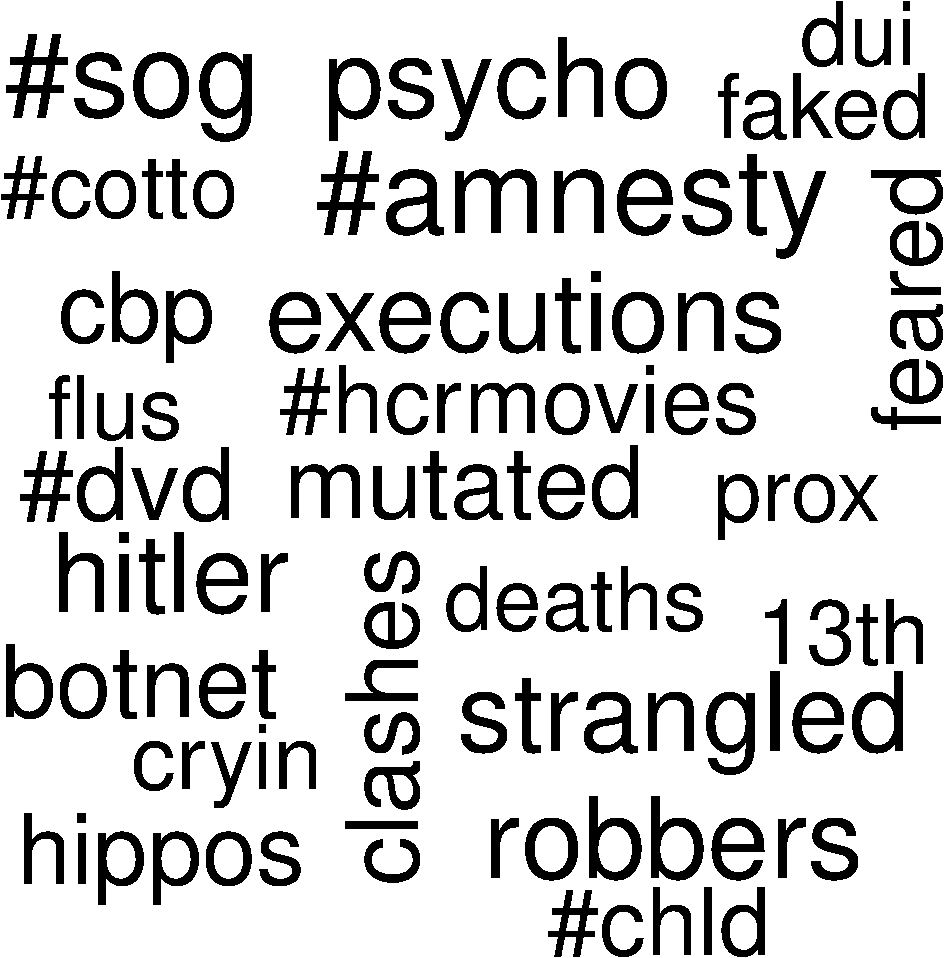
\includegraphics[scale=0.2]{pics/fear.pdf} \\
anger & anticipation & disgust & fear\\[1mm] 
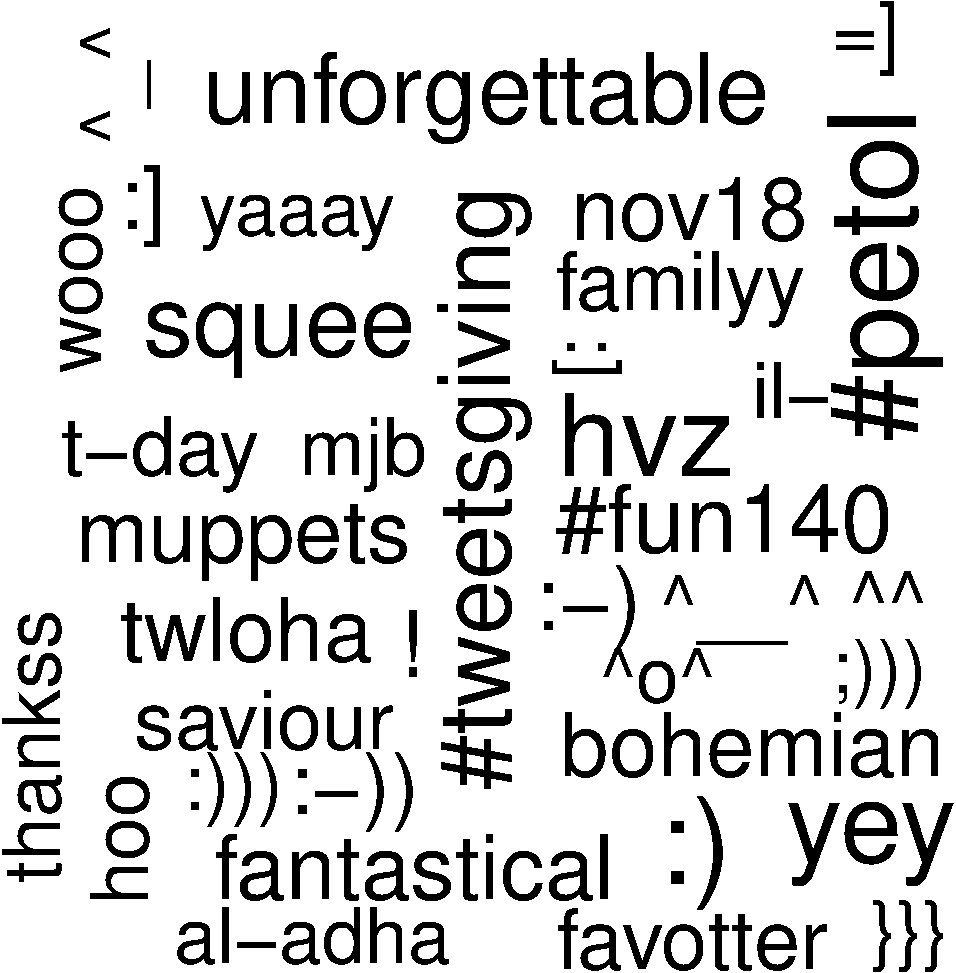
\includegraphics[scale=0.2]{pics/joy.pdf} & 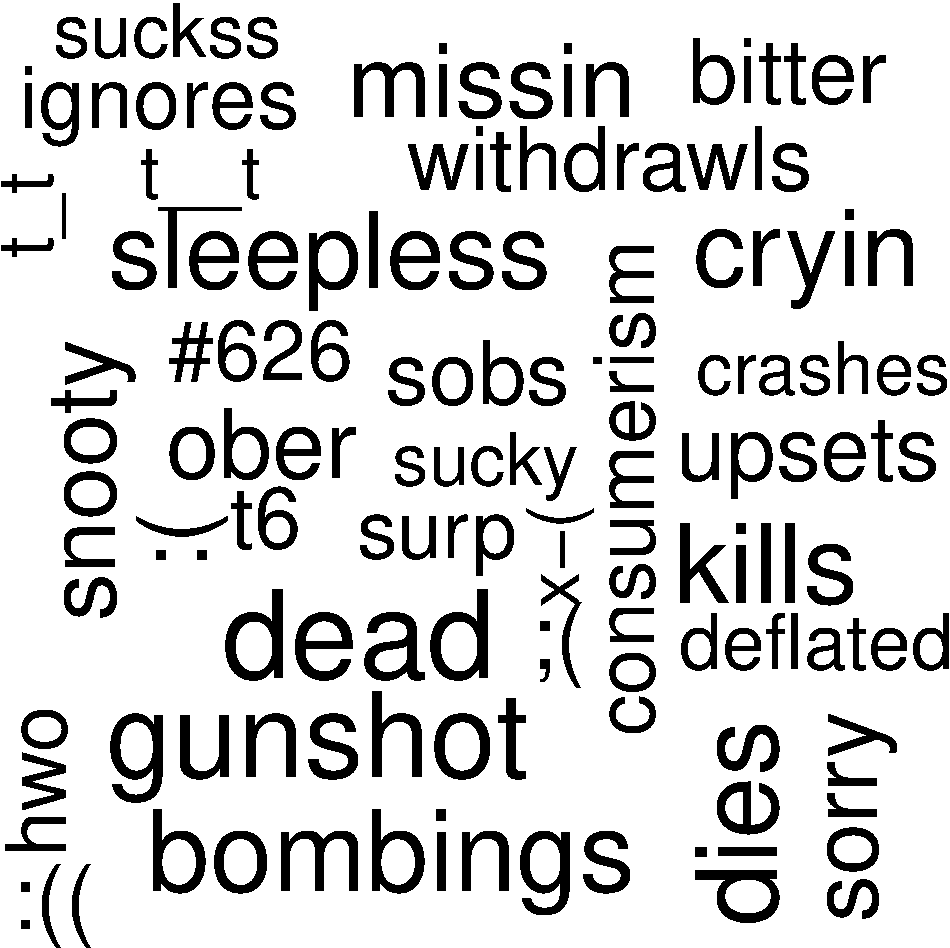
\includegraphics[scale=0.2]{pics/sadness.pdf} & 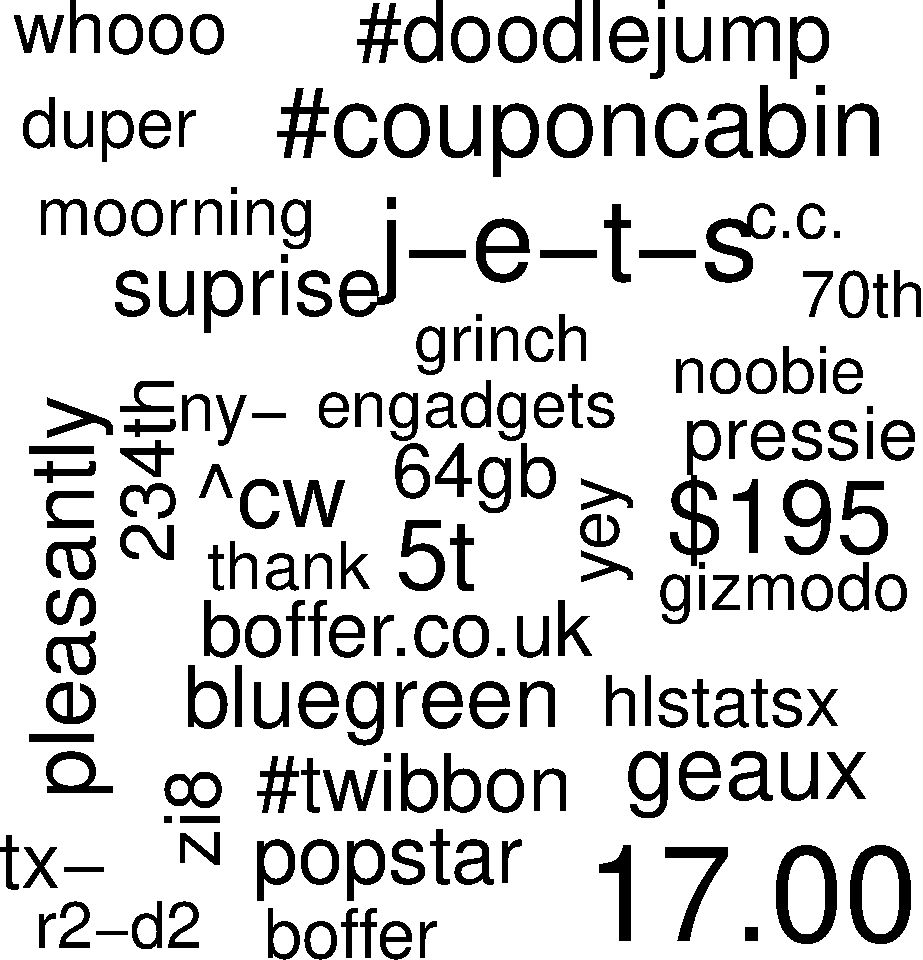
\includegraphics[scale=0.2]{pics/surprise.pdf} & 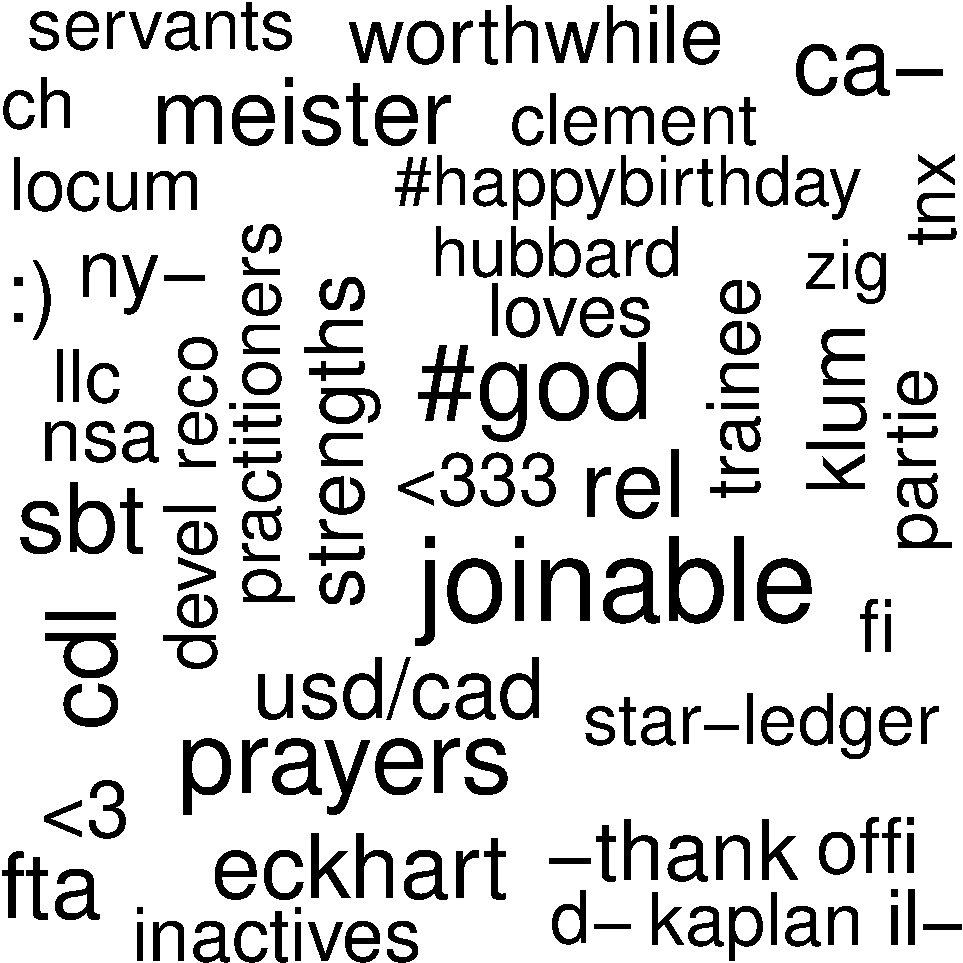
\includegraphics[scale=0.2]{pics/trust.pdf} \\
joy & sadness & surprise & trust\\
\end{tabular}}
\end{center}
\end{figure}

\end{scriptsize}
\end{frame}

\begin{frame}{Other Applications of TCM}
\begin{scriptsize}
\begin{block}{Transfer Learning for PLI}
\begin{itemize}
 \item What if we don't have a seed lexicon?
 \item We can train a \textbf{message-level classifier} $f_M$ from a corpus of sentiment annotated tweets $\mathcal{C}_L$ and deploy it on words found in a \textbf{corpus of unlabelled tweets} represented by tweet centroids.
 \item Tweets are represented by  \textbf{sparse vectors} using unigrams, Brown clusters, and POS tags.
 \item Note that tweets and words reside in the \textbf{same feature space}.

 \end{itemize}

\begin{table}[htbp]
\begin{tabular}{l|ll}
\hline \hline
\multicolumn{3}{c}{AUC} \\
\hline \hline
Source Dataset & PMI-SO & TCM  \\ \hline
Sanders & 0.757 &  \textbf{0.864} \\ 
6HumanCoded & 0.861 & \textbf{0.930}  \\ 
SemEval & 0.858 & \textbf{0.916}   \\ \hline
\end{tabular}
\caption{Word-level Polarity Classification Results for the AFINN lexicon.}
\end{table}
\end{block}

\end{scriptsize}
\end{frame}



\section{Distant Supervision}

\begin{frame}{Lexical-based Distant Supervision}
\begin{scriptsize}
\begin{itemize}
\item Lexicons showed to be \textbf{useful features} for MPC.
\item But we \textbf{still need labelled tweets} for training a message-level classifier.
\item We will try to \textbf{directly use} lexical knowledge for training message-level classifiers.
\item We propose two \textbf{distant supervision} models: \textbf{Partitioned Tweet Centroids} and \textbf{Annotate-Sample-Average (ASA)}.

 \item Proposed methods generate positive and negative training instances by \textbf{averaging} tweets containing words with the \textbf{same} polarity.

\end{itemize}
\end{scriptsize}

\end{frame}



\begin{frame}{Lexical Polarity Hypothesis}
\begin{scriptsize}
\begin{itemize}

\item A tweet containing a word with a certain polarity is more likely to express the \textbf{same polarity} than the \textbf{opposite} $p_d>0.5$ (Bernoulli experiment).




 \begin{figure}[htb]
\begin{center}
\scalebox{0.18}{
\begin{tabular}{cc}
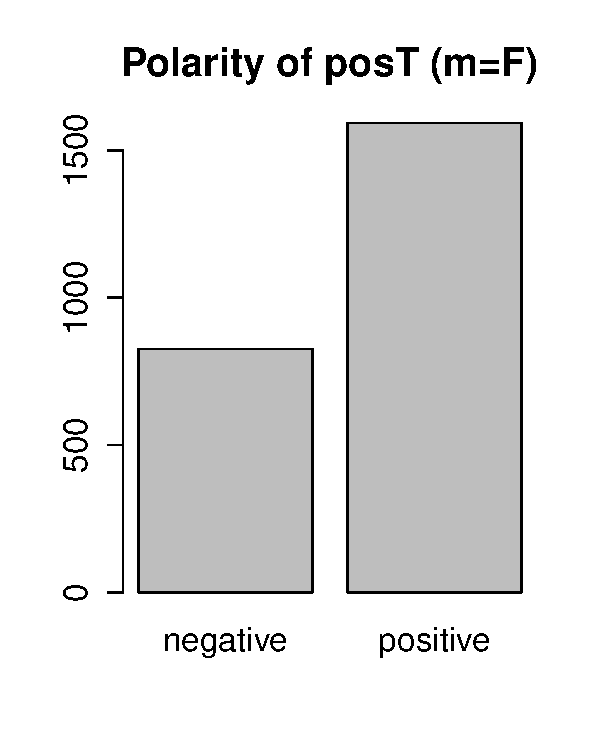
\includegraphics{pics/posTmF.pdf} &  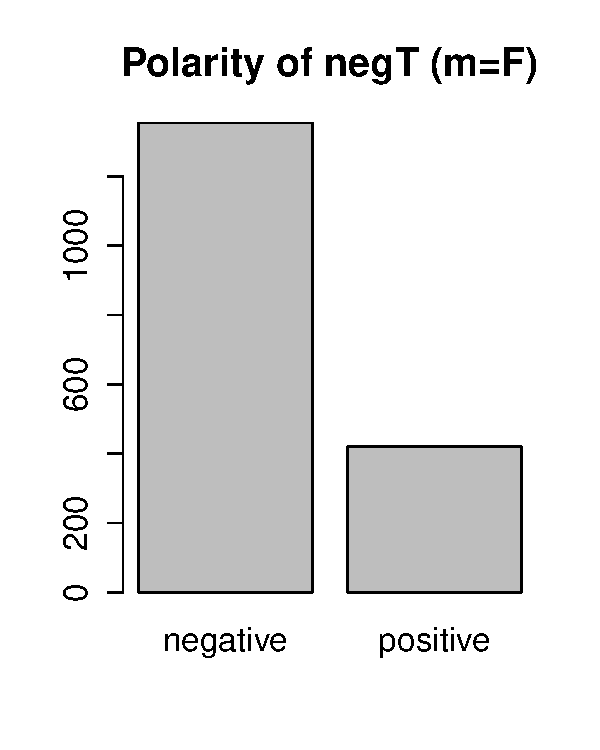
\includegraphics{pics/negTmF.pdf}  \\
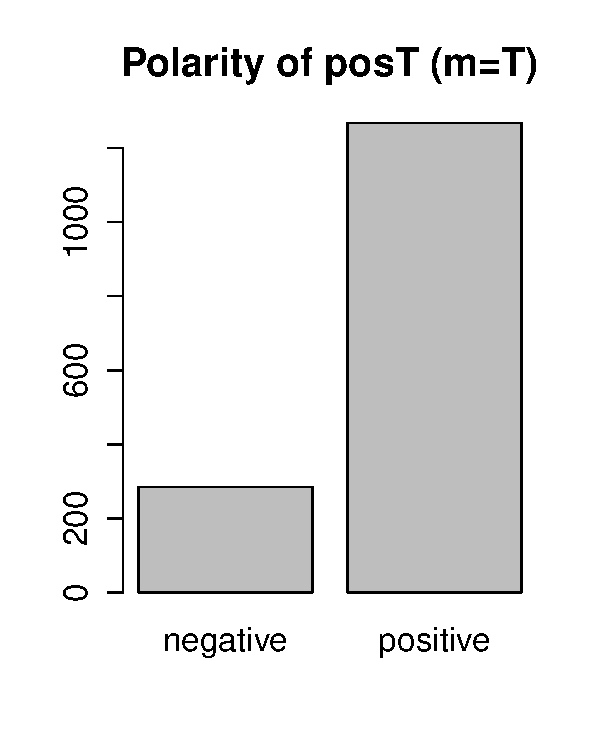
\includegraphics{pics/posTmT.pdf} &  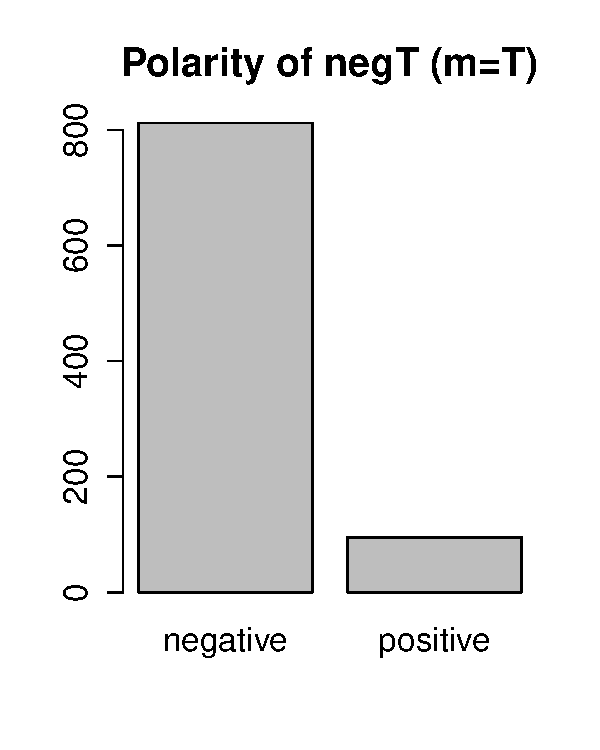
\includegraphics{pics/negTmT.pdf}  \\
\end{tabular}}
\label{fig:barplots}
\end{center}
\end{figure}

\item The opposite polarity may also be expressed due to the presence of  \textbf{negation}, \textbf{sarcasm}, or other opinion words with the \textbf{opposite} polarity.

\end{itemize}
\end{scriptsize}

\end{frame}


\begin{frame}{Why Averaging?}
\begin{scriptsize}
\begin{itemize}
\item Averaging multiple tweets with words with the same polarity \textbf{increases} the confidence of generating instances located in the \textbf{region} of the desired polarity.
\item We assume that the average tweet will behave similarly to the \textbf{majority}.
\item Probability that the \textbf{majority} of the tweets sampled from a collection of tweets with at least one word with the target polarity have the desired polarity:
\begin{displaymath}
 P(M) = \sum_{i=\lfloor \frac{a}{2}\rfloor +1}^a \binom a i  p_d^i(1-p_d)^{a-i}
\end{displaymath}
         
\begin{table}
\begin{center}
\scalebox{0.7}{
\begin{tabular}{|l|l|l|l|l|}
\hline
 & $p_d = 0.6$ & $p_d = 0.7$ & $p_d = 0.8$ & $p_d = 0.9$ \\  \hline
$a = 3$ &  0.648 & 0.784 & 0.896 & 0.972 \\
$a = 5$ & 0.683 & 0.837 & 0.942 & 0.991 \\ 
$a = 10$ & 0.633 & 0.850 & 0.967 & 0.998 \\ 
$a = 50$ & 0.902 & 0.998 & 1 & 1 \\ 
$a = 100$ & 0.973 & 1 & 1 & 1 \\ 
$a = 500$ & 1 & 1 & 1 & 1 \\ 
$a = 1000$ & 1 & 1 & 1 & 1 \\ \hline
\end{tabular}}
\end{center}
\end{table}
\item $P(M) > p_d$, when $a \geq 3$ and $p_d \geq 0.5$.  This is analogous to the \textbf{Condorcet's Jury Theorem}!!
\end{itemize}
\end{scriptsize}

\end{frame}



\begin{frame}{TCM for message-level classification}
\begin{scriptsize}
\begin{itemize}
\item TCM can be used as a \textbf{distant supervision} model for MPC.
\item We use a \textbf{word-level} classifier $f_W$ trained with TCM vectors calculated from $\mathcal{C}_U$ labelled by a \textbf{polarity lexicon} $\mathcal{L}$ (AFINN). 
\item The classifier is deployed on the target tweets represented by \textbf{sparse vectors}.
\item The number of labelled words for training $f_W$ is \textbf{limited} to the number of words from $\mathcal{L}$.
\item TCM is \textbf{not capable} of exploiting large collections of unlabelled tweets for producing training datasets larger than the size of $\mathcal{L}$. 
\end{itemize}
\end{scriptsize}
\end{frame}

\begin{frame}{Partitioned TCM}
\begin{scriptsize}
\begin{itemize}
\item We propose a modification of our method for \textbf{increasing} the number labelled instances it produces. 
\item  The word-tweet set $\mathcal{M}(w)$ for each word from the lexicon ($w \in\mathcal{L}$) is \textbf{partitioned} into smaller disjoint subsets $\mathcal{M}(w)_1, \dots \mathcal{M}(w)_z$ of a fixed size determined by a parameter $p$. 
\item We calculate one tweet centroid vector $\overrightarrow{w}$ for \textbf{each partition} labelled according to $\mathcal{L}$.
\end{itemize}
\end{scriptsize}
\end{frame}


\begin{frame}{Baselines}
\begin{scriptsize}
\begin{block}{Emoticon-Annotation Approach (EAA)}
\begin{itemize}
\item Labels tweets with positive or negative emoticons according to the emoticon's polarity after removing the emoticon from the message.
\item  Tweets containing both positive and negative emoticons are \textbf{discarded}.
\end{itemize}
\end{block}

\begin{block}{Lexicon-annotation approach (LAA)}
\begin{itemize}
\item Uses a given polarity lexicon $\mathcal{L}$.
\item Tweets with at least one positive word and no negative word are labelled \textbf{positive}.
\item Tweets with at least one negative word and no positive word are labelled \textbf{negative}.
\end{itemize}
\end{block}

\end{scriptsize}
\end{frame}


\begin{frame}{Instances Generated by Distant Supervision Models}
We use 10 collections of 2 million tweets as source corpora.
\begin{table}
\begin{center}
\scalebox{0.7}{
\begin{tabular}{l|ll@{\hspace{0.1cm}}|ll@{\hspace{0.1cm}}|ll@{\hspace{0.1cm}}}
\hline
 & Avg. Positive & (\%) & Avg. Negative & (\%) & Avg. Total & (\%) \\ \hline
EAA & $130,641$ & (6.5\%) & $21,537$ & (1.1\%) & $152,179$ & (7.6\%) \\ 
LAA & $681,531$ & (34.1\%) & $294,177$ & (14.7\%) & $975,708$ & (48.8\%) \\ 
TCM & $1537$ & (0.05\%) & $951$ & (0.08\%) & $2488$ & (0.12\%) \\ 
TCM ($p$=5) & $276,696$ & (13.8\%) & $149,989$ & (7.5\%) & $426,684$ & (21.3\%) \\ 
TCM ($p$=10) & $138,596$ & (6.9\%) & $75,390$ & (3.8\%) & $213,986$ & (10.7\%) \\ 
TCM ($p$=20) & $69,518$  & (3.5\%) & $38,044$ & (1.9\%) & $107,563$ & (5.4\%) \\ 
TCM ($p$=50)& $32,231$ & (1.6\%) & $17,950$ & (0.9\%) & $50,181$ & (2.5\%) \\ 
TCM ($p$=100)& $14,338$ & (0.7\%) & $8357$ & (0.4\%) & $22,695$ & (1.1\%) \\ \hline
\end{tabular}}
\end{center}
\end{table} 


\end{frame}




\begin{frame}{TCM for MPC}

\begin{table}[htbp]
\begin{center}
\scalebox{0.8}{
\begin{tabular}{l|ll@{\hspace{0.1cm}}l@{\hspace{0.1cm}}|ll@{\hspace{0.1cm}}l@{\hspace{0.1cm}}|ll@{\hspace{0.1cm}}l@{\hspace{0.1cm}}}
\hline
 & \multicolumn{3}{c|}{6HumanCoded} & \multicolumn{3}{c|}{Sanders} & \multicolumn{3}{c}{SemEval} \\ \hline
EAA & 0.805 $\pm$ 0.005 & = & - & 0.800 $\pm$ 0.017 & = & +& 0.802  $\pm$ 0.006 & = & - \\ 
LAA & 0.809 $\pm$ 0.001 & + & = & 0.778 $\pm$ 0.002 & - & = & 0.814  $\pm$ 0.000 &+ & =\\ \hline
TCM & 0.776 $\pm$ 0.004 &-&-& 0.682 $\pm$ 0.024 &-&-& 0.779  $\pm$ 0.008 &-&-\\ 
TCM ($p$=5) & 0.834 $\pm$ 0.002 & + & +& 0.807 $\pm$ 0.008 &= & +& 0.833  $\pm$ 0.002 &+&+ \\ 
TCM ($p$=10) & 0.845 $\pm$ 0.003 & + & +& \textbf{0.817} $\pm$ 0.006 &+ & +& 0.841  $\pm$ 0.002 &+ & +\\ 
TCM ($p$=20) & \textbf{0.850} $\pm$ 0.003 &+ & +& 0.815 $\pm$ 0.011 &+ & +& \textbf{0.844}  $\pm$ 0.003 & + & +\\ 
TCM ($p$=50) & 0.844 $\pm$ 0.004 & + & +& 0.785 $\pm$ 0.010 & - & +& 0.836  $\pm$ 0.004 & + & +\\ 
TCM ($p$=100) & 0.829 $\pm$ 0.003 & + & +& 0.752 $\pm$ 0.019 & - & -& 0.821  $\pm$ 0.004 & + & +\\ \hline
\end{tabular}}
\end{center}
\caption{Message-level Polarity Classification Results. Best results per column are given in bold.}
\label{tab:messclas}
\end{table}
\end{frame}



\begin{frame}{Annotate-Sample-Average (ASA)}
\begin{scriptsize}
 \begin{itemize}
 \item Partitioned TCM can generate \textbf{very large} training datasets.
 \item TCM instances are obtained by averaging tweets containing \textbf{the same word}.
 \item What if we average random tweets containing \textbf{different words} with the same polarity?
 \item What if we can define the \textbf{number of instances} to generate?
 \item This could be useful for creating \textbf{compact and balanced} training datasets. 
 
 \end{itemize}
 
  
 
\end{scriptsize} 
\end{frame}

\begin{frame}{Annotate-Sample-Average (ASA)}
\begin{scriptsize}
 \begin{itemize}
 \item \textbf{Annotation}: every time a word from $\mathcal{L}$  is found, the  tweet is added to sets \textbf{posT} or \textbf{negT} (depending on the polarity).
 \item Tweets with both positive and negative words will be discarded if the flag $m$ is set, and will be simultaneously added to both \textbf{posT} and \textbf{negT} otherwise. 
 
 \item Tweets are likely to contain words with the \textbf{opposite polarity}: we believe that unsetting the flag will produce instances with better \textbf{generalisation} properties. 
 \item \textbf{Sample}: randomly sample with replacement $a$ tweets from either \textbf{posT} or \textbf{negT} for each generated instance. 
 \item \textbf{Averaging}: average and label sampled feature vectors.
 \item We create balanced training datasets with size equal to 1\% of the size of the source corpus ($20,000$ in our experiments).
 \end{itemize}
  
\end{scriptsize} 
\end{frame}

\begin{frame}{ASA results}

\begin{table}[htb]
\begin{center}
\scalebox{0.6}{
\begin{tabular}{l|ll@{\hspace{0.1cm}}l@{\hspace{0.1cm}}l@{\hspace{0.1cm}}l@{\hspace{0.1cm}}|ll@{\hspace{0.1cm}}l@{\hspace{0.1cm}}l@{\hspace{0.1cm}}l@{\hspace{0.1cm}}|ll@{\hspace{0.1cm}}l@{\hspace{0.1cm}}l@{\hspace{0.1cm}}l@{\hspace{0.1cm}}l@{\hspace{0.1cm}}l@{\hspace{0.1cm}}l@{\hspace{0.1cm}}l@{\hspace{0.1cm}}}
\hline
 & \multicolumn{ 5}{c|}{6HumanCoded} & \multicolumn{5}{c|}{Sanders} & \multicolumn{5}{c}{SemEval} \\ \hline
EAA\_U & 0.805 $\pm$ 0.005 & = & = & - & - & 0.800 $\pm$ 0.017 & = & = & + & + & 0.802 $\pm$ 0.006 & = & + & - & - \\ 
EAA\_B &  0.809 $\pm$ 0.001 & = & = & = & = & 0.795 $\pm$ 0.016 & = & = & + & + & 0.798 $\pm$ 0.007 & - & = & - & - \\ 
LAA\_U & 0.809 $\pm$ 0.001 & + & = & = & = & 0.778 $\pm$ 0.002 & - & - & = & = & 0.814 $\pm$ 0.000 & + & + & = & = \\ 
LAA\_B & 0.809 $\pm$ 0.001 & + & = & = & = & 0.778 $\pm$ 0.003 & - & - & = & = & 0.813 $\pm$ 0.001 & + & + & = & = \\ \hline
ASA ($a=1$, $m=T$) & 0.806 $\pm$ 0.003 & = & = & - & - & 0.786 $\pm$ 0.007 & - & - & + & +  & 0.808 $\pm$ 0.002 & + & + & - & -  \\ 
ASA ($a=5$, $m=T$)  & 0.809 $\pm$ 0.002 & = & = & = & =  & 0.787 $\pm$ 0.005 & - & = & + & +  & 0.810 $\pm$ 0.003 & + & + & - & -  \\ 
ASA ($a=10$, $m=T$) & 0.804 $\pm$ 0.001 & = & - & - & -  & 0.776 $\pm$ 0.008 & - & - & = & =  & 0.806 $\pm$ 0.003 & + & + & - & -  \\ 
ASA ($a=50$, $m=T$) & 0.756 $\pm$ 0.003 & - & - & - & -  & 0.697 $\pm$ 0.005 & - & - & - & -  & 0.763 $\pm$ 0.002 & - & - & - & - \\ 
ASA ($a=100$, $m=T$)  & 0.729 $\pm$ 0.002 & - & - & - & -  & 0.672 $\pm$ 0.006 & - & - & - & -  & 0.739 $\pm$ 0.002 & - & - & - & -  \\ 
ASA ($a=500$, $m=T$)  & 0.696 $\pm$ 0.003 & - & - & - & -  & 0.642 $\pm$ 0.008 & - & - & - & -  & 0.707 $\pm$ 0.005 & - & - & - & -  \\ 
ASA ($a=1000$, $m=T$) & 0.690 $\pm$ 0.004 & - & - & - & -  & 0.637 $\pm$ 0.008 & - & - & - & -  & 0.701 $\pm$ 0.006 & - & - & - & -  \\ \hline
ASA ($a=1$, $m=F$) & 0.793 $\pm$ 0.005 & - & - & - & -  & 0.762 $\pm$ 0.016 & - & - & - & -  & 0.787 $\pm$ 0.007 & - & - & - & -  \\ 
ASA ($a=5$, $m=F$)  & 0.837 $\pm$ 0.004 & + & + & + & +  & 0.807 $\pm$ 0.010 & = & = & + & +  & 0.833 $\pm$ 0.003 & + & + & + & +  \\ 
ASA ($a=10$, $m=F$) & \textbf{0.845} $\pm$ 0.001 & + & + & + & +  & \textbf{0.812} $\pm$ 0.015 & + & + & + & +  & \textbf{0.840} $\pm$ 0.003 & + & + & + & +  \\ 
ASA ($a=50$, $m=F$) & 0.815 $\pm$ 0.003 & + & + & + & +  & 0.759 $\pm$ 0.006 & - & - & - & -  & 0.810 $\pm$ 0.004 & + & + & - & - \\ 
ASA ($a=100$, $m=F$)  & 0.781 $\pm$ 0.003 & - & - & - & -  & 0.720 $\pm$ 0.007 & - & - & - & -  & 0.779 $\pm$ 0.004 & - & - & - & -  \\ 
ASA ($a=500$, $m=F$)  & 0.723 $\pm$ 0.002 & - & - & - & -  & 0.670 $\pm$ 0.008 & - & - & - & -  & 0.729 $\pm$ 0.005 & - & - & - & -  \\ 
ASA ($a=1000$, $m=F$) & 0.712 $\pm$ 0.002 & - & - & - & -  & 0.665 $\pm$ 0.007 & - & - & - & -  & 0.721 $\pm$ 0.005 & - & - & - & -  \\ 
\end{tabular}}
\end{center}
\caption{AUC measure for different distant supervision models. Best results per column are given in bold. }
\label{tab:resA}
\end{table} 
  
\end{frame}

\begin{frame}{ASA results}

\begin{table}[htb]
\begin{center}
\scalebox{0.6}{
\begin{tabular}{l|ll@{\hspace{0.1cm}}l@{\hspace{0.1cm}}l@{\hspace{0.1cm}}l@{\hspace{0.1cm}}|ll@{\hspace{0.1cm}}l@{\hspace{0.1cm}}l@{\hspace{0.1cm}}l@{\hspace{0.1cm}}|ll@{\hspace{0.1cm}}l@{\hspace{0.1cm}}l@{\hspace{0.1cm}}l@{\hspace{0.1cm}}l@{\hspace{0.1cm}}l@{\hspace{0.1cm}}l@{\hspace{0.1cm}}l@{\hspace{0.1cm}}}
\hline
 & \multicolumn{ 5}{c|}{6HumanCoded} & \multicolumn{5}{c|}{Sanders} & \multicolumn{5}{c}{SemEval} \\ \hline
EAA\_U & 0.576 $\pm$ 0.007 & = & - & - & - & 0.506 $\pm$ 0.018 & = & - & - & - & 0.591 $\pm$ 0.018 & = & - & - & - \\ 
EAA\_B & 0.735 $\pm$ 0.008 & + &  = & + & + & 0.709 $\pm$ 0.018 & + & = & = & = & 0.711 $\pm$ 0.006 & + & = & - & = \\ 
LAA\_U & 0.729 $\pm$ 0.004 & + & - & = & + & 0.711 $\pm$ 0.003 & + & = & = & + & 0.725 $\pm$ 0.002 & + & + & = & + \\ 
LAA\_B & 0.719 $\pm$ 0.002 & + & - & - & = & 0.703 $\pm$ 0.004 & + & = & - & = & 0.712 $\pm$ 0.002 & + & = & - & = \\ \hline
ASA ($a=1$, $m=T$) & 0.734 $\pm$ 0.005 & + & = & + & + & 0.721 $\pm$ 0.010 & + & + & + & +  & 0.724 $\pm$ 0.004 & + & + & = & +  \\ 
ASA ($a=5$, $m=T$)  & 0.745 $\pm$ 0.005 & + & + & + & + & 0.723 $\pm$ 0.010 & + & + & + & +  & 0.722 $\pm$ 0.006 & + & + & = & +  \\ 
ASA ($a=10$, $m=T$) & 0.737 $\pm$ 0.003 & + & = & + & + & 0.703 $\pm$ 0.011 & + & = & - & =  & 0.708 $\pm$ 0.007 & + & - & - & =  \\ 
ASA ($a=50$, $m=T$) & 0.693 $\pm$ 0.003 & + & - & - & - & 0.643 $\pm$ 0.004 & + & - & - & -  & 0.639 $\pm$ 0.006 & + & - & - & - \\ 
ASA ($a=100$, $m=T$)  & 0.672 $\pm$ 0.004 & + & - & - & - & 0.620 $\pm$ 0.005 & + & - & - & -  & 0.607 $\pm$ 0.006 & + & - & - & -  \\ 
ASA ($a=500$, $m=T$)  & 0.638 $\pm$ 0.004 & + & - & - & - & 0.599 $\pm$ 0.008 & + & - & - & - & 0.563 $\pm$ 0.005 & - & - & - & -  \\ 
ASA ($a=1000$, $m=T$) & 0.635 $\pm$ 0.004 & + & - & - & - & 0.594 $\pm$ 0.010 & + & - & - & -  & 0.554 $\pm$ 0.003 & - & - & - & -  \\ \hline
ASA ($a=1$, $m=F$) & 0.717 $\pm$ 0.007 & + & - & - & = & 0.691 $\pm$ 0.013 & + & - & - & -  & 0.699 $\pm$ 0.008 & + & - & - & -  \\ 
ASA ($a=5$, $m=F$)  & 0.755 $\pm$ 0.004 & + & + & + & + & 0.730 $\pm$ 0.008 & + & + & + & +  & 0.735 $\pm$ 0.005 & + & + & + & +  \\ 
ASA ($a=10$, $m=F$) & \textbf{0.761} $\pm$ 0.003 & + & + & + & + & \textbf{0.735} $\pm$ 0.015 & + & + & + & +  & \textbf{0.742} $\pm$ 0.006 & + & + & + & +  \\ 
ASA ($a=50$, $m=F$) & 0.749 $\pm$ 0.004 & + & + & + & + & 0.673 $\pm$ 0.005 & + & - & - & - & 0.699 $\pm$ 0.009 & + & - & - & - \\ 
ASA ($a=100$, $m=F$)  & 0.717 $\pm$ 0.003 & + & - & - & - & 0.645 $\pm$ 0.006 & + & - & - & -  & 0.664 $\pm$ 0.005 & + & - & - & -  \\ 
ASA ($a=500$, $m=F$)  & 0.665 $\pm$ 0.002 & + & - & - & - & 0.621 $\pm$ 0.007 & + & - & - & -  & 0.621 $\pm$ 0.004 & + & - & - & -  \\ 
ASA ($a=1000$, $m=F$) & 0.653 $\pm$ 0.003 & + & - & - & - & 0.619 $\pm$ 0.007 & + & - & - & -  & 0.613 $\pm$ 0.002 & + & - & - & - \\ 
\end{tabular}}
\end{center}
\caption{Macro-averaged F1 measure for different distant supervision models. Best results per column are given in bold. }
\label{tab:resF}
\end{table}
 
 
\end{frame}



\section{Conclusions}

\begin{frame}{Conclusions}
\begin{scriptsize}
\begin{itemize}
\item The methods developed in this thesis can be used to \textbf{acquire} and \textbf{exploit} lexical knowledge for Twitter sentiment analysis under \textbf{label sparsity conditions}. 

\item We proposed two methods (Word Sentiment Associations and TCM) for building Twitter-specific \textbf{opinion lexicons} (acquisition of lexical knowledge).

\item These methods could be used to create \textbf{domain-specific} lexicons.
\item They could also be used to study the \textbf{dynamics} of opinion-words.
\item Future work: try \textbf{non-linear representations} on TCM (Auto-Encoders or RBM).

\end{itemize}
\end{scriptsize}

\end{frame}



\begin{frame}{Conclusions}
\begin{scriptsize}
\begin{itemize}
\item  We proposed two \textbf{distant supervision methods} (TCM and ASA) that outperformed LAA and EAA for MPC.

\item TCM is a \textbf{unified model} for message-level and word-level sentiment classification.


\item Future work: subjectivity, emotions, handle negations, non-linear representations and deep networks. Volunteers?
\end{itemize}
\end{scriptsize}

\end{frame}

\begin{frame}{Publications}
\begin{tiny}

\begin{enumerate}

\item F. Bravo-Marquez, E. Frank, and B. Pfahringer \textit{Positive, Negative, or Neutral: Learning an Expanded Opinion Lexicon from Emoticon-annotated Tweets}, In \textit{IJCAI '15: Proceedings of the 24th International Joint Conference on Artificial Intelligence}. Buenos Aires, Argentina 2015.

\item F. Bravo-Marquez, E. Frank, and B. Pfahringer \textit{From Unlabelled Tweets to Twitter-specific Opinion Words}, In \textit{SIGIR '15: Proceedings of the 38th International ACM SIGIR Conference on Research \& Development in Information Retrieval}. Santiago, Chile 2015. 


\item F. Bravo-Marquez, E. Frank, and B. Pfahringer \textit{Building a Twitter Opinion Lexicon from Automatically-annotated Tweets}, In \textit{Knowledge-Based Systems}. Volume 108, 15 September 2016, Pages 65 -– 78.


\item F. Bravo-Marquez, E. Frank, and B. Pfahringer \textit{Annotate-Sample-Average (ASA): A New Distant
Supervision Approach for Twitter Sentiment Analysis}, In \textit{ECAI'16: Proceedings of the biennial European Conference  on Artificial Intelligence}. The Hague, Netherlands 2016.


\item F. Bravo-Marquez, E. Frank, and B. Pfahringer \textit{From opinion lexicons to sentiment classification of
tweets and vice versa: a transfer learning approach}, In \textit{WI'16: Proceedings of the IEEE/WIC/ACM International Conference on Web Intelligence}. Omaha, Nebraska, USA 2016.


\item F. Bravo-Marquez, E. Frank, S. Mohammad, and B. Pfahringer \textit{Determining Word--Emotion Associations from Tweets by Multi-Label Classification}, In \textit{WI'16: Proceedings of the IEEE/WIC/ACM International Conference on Web Intelligence}. Omaha, Nebraska, USA 2016.


\end{enumerate}

\end{tiny}
\end{frame}


\begin{frame}
\frametitle{Questions?}
%\vspace{1.5cm}
\begin{center}\LARGE Thanks for your Attention!\\ \#ThankYouHeaps \\ \#GraciasTotales \end{center}

\begin{columns}
\begin{column}{0.55\textwidth}
\begin{block}{Acknowledgements}
\begin{itemize}\tiny
	\item University of Waikato Doctoral Scholarship
	\item Machine Learning Group at the University of Waikato
	
\end{itemize}
\end{block}
\end{column}
\begin{column}{0.45\textwidth}
\vspace{1.5cm}

\begin{figure}[h!]
	\centering
	\includegraphics[scale=0.3]{../../img/waikato.png}
\end{figure}
\end{column}
\end{columns}

\end{frame}

\begin{frame}[allowframebreaks]\scriptsize
\frametitle{References}
\bibliography{../bio}
\bibliographystyle{apalike}
%\bibliographystyle{flexbib}
\end{frame}  


%%%%%%%%%%%%%%%%%%%%%%%%%%%

\end{document}
